%%%% ijcai19-multiauthor.tex

\typeout{IJCAI-19 Multiple authors example}

% These are the instructions for authors for IJCAI-19.

\documentclass{article}
\pdfpagewidth=8.5in
\pdfpageheight=11in
% The file ijcai19.sty is NOT the same than previous years'
\usepackage{ijcai19}

% Use the postscript times font!
\usepackage{times}
\usepackage{soul}
\usepackage{url}
\usepackage[hidelinks]{hyperref}
\usepackage[utf8]{inputenc}
\usepackage[small]{caption}
\usepackage{graphicx}
\usepackage{amsmath}
\usepackage{booktabs}
\usepackage{algorithm}
\usepackage{algorithmic}
\urlstyle{same}

% the following package is optional:
%\usepackage{latexsym} 

% Following comment is from ijcai97-submit.tex:
% The preparation of these files was supported by Schlumberger Palo Alto
% Research, AT\&T Bell Laboratories, and Morgan Kaufmann Publishers.
% Shirley Jowell, of Morgan Kaufmann Publishers, and Peter F.
% Patel-Schneider, of AT\&T Bell Laboratories collaborated on their
% preparation.

% These instructions can be modified and used in other conferences as long
% as credit to the authors and supporting agencies is retained, this notice
% is not changed, and further modification or reuse is not restricted.
% Neither Shirley Jowell nor Peter F. Patel-Schneider can be listed as
% contacts for providing assistance without their prior permission.

% To use for other conferences, change references to files and the
% conference appropriate and use other authors, contacts, publishers, and
% organizations.
% Also change the deadline and address for returning papers and the length and
% page charge instructions.
% Put where the files are available in the appropriate places.

\title{ An Analysis of Different Reinforcement Learning Techniques on a Custom Implementation of a Blokus Gym Environment }

\author{
Andréanne Lemay$^1$\and
Francis Granger$^1$\And
Yoan Gauthier$^1$\\
\affiliations
$^1$École Polytechnique de Montréal\\
\emails
\{andreanne.lemay, francis.granger, yoan.gauthier\}@polymtl.ca
}

\begin{document}
\maketitle


\begin{abstract}
  Presentation des resultats et petite entree vrm cheasy af yoan est sexy!!!
\end{abstract}

\section{Introduction}

Recent superhuman performance achievements in the game of Go by \cite{alphaGo} and also in chess with \cite{alphaZero} have helped cause a huge spike in reinforcement learning use cases. These methods use a general purpose Monte Carlo Tree Search and self play algorithms to maximize the expected outcome. On another approach, \cite{rainbow} tries to boost the performance of all the DQN alternatives, but has mostly been tested on Atari games with a much simpler action space than the previous board games, for exemple, the game of Pong only has two possible moves at almost every moment. This paper examines the performance of Rainbow on the board game of Blokus which has a good in between number of actions per move.

\subsection{The Game of Blokus}

Blokus\footnote{\url{https://en.wikipedia.org/wiki/Blokus}} is a French board game that was invented in 2000. In the original game, every player gets 21 pieces, each consisting of 1 to 5 tiles. At each turn, the player is allowed to play one piece and the new tile can only be placed from corners to corners from the current player tiles. This means that the new tiles cannot touch any side of any other tiles from the current player, it however can touch anything from other players. An example is shown in figure \ref{fig:moves}. This is where the name "block us" comes from, the idea is to block the corners of the other players resulting in less possible moves for them. The game finishes when everyone is out of moves and the winner is the one that covers the biggest area. In other words, the one that placed the most tiles, not necessarily pieces.

\begin{figure}[h!]
  \caption{A good and a bad move}
  \label{fig:moves}
\begin{minipage}{6in}
  \hspace*{.3in}
  \raisebox{-0.25\height}{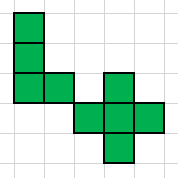
\includegraphics[height=1.25in]{good_move.png}}
  \hspace*{.2in}
  \raisebox{-0.25\height}{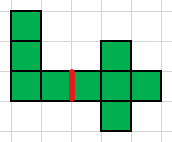
\includegraphics[height=1in]{bad_move.png}}
\end{minipage}
\end{figure}

\subsection{The DQN Algorithms}

The Deep Q-Learning method was brought by \cite{rainbow} to solve many reinforcement learning problems. Multiple researches have been done after that to try to improve the efficiency on multiple different use cases and environments.
\\\\ % TODO MAYBE REMOVE LATER

This paper focuses on the Rainbow algorithm which combines:
\begin{itemize}
\item Regular DQN
\item Double DQN (DDQN)
\item Prioritized DDQN
\item Dueling DDQN
\item Distributional DQN
\item Noisy DQN
\end{itemize}
All those, to create the best possible results.

\section{Methodology}

This section details how the action and observation spaces are organized over multiple environments and the model is constructed.

\subsection{Observation and Action Spaces}

For this task we created 9 Open AI \footnote{\url{https://openai.com/}} Gym Environments \footnote{\url{https://gym.openai.com/docs/}} consisting of three different boards:
\begin{itemize}
\item Simple: a smaller representation of the game for faster training time and a proof of concept. This board is only for two players and all the 5 tiles pieces have been removed.
\item Duo: this is the official Blokus duo game
\item Hard: this is also the official and original Blokus game
\end{itemize}

Each with the possibility of being played against three different bots: 
\begin{itemize}
\item Random: selects randomly between all the possible moves
\item Greedy: maximizes the number of tiles and then the number of newly blocked and opened corners)
\item Minimax: same as greedy but with 3 recursive calls
\end{itemize}

The representation of the various boards available can be found in \ref{tab:boards}
\begin{table}
\centering
\begin{tabular}{llll}
\hline
 & Simple [\ref{fig:simpleBoard}] & Duo [\ref{fig:duoBoard}] & Hard [\ref{fig:hardBoard}] \\
\hline
Board Size & $7\times7$ & $14\times14$ & $21\times21$ \\
Players & 2 & 2 & 4 \\
Observations & 147 & 588 & 2205 \\
Pieces & 12 & 21 & 21 \\
Actions & 919 & 13 729 & 33 854 \\
Mean per turn & 19 & 160 & 205 \\
\hline
\end{tabular}
\caption{Difficulties per board type}
\label{tab:boards}
\end{table}

\begin{figure}[h!]
\centering
  \caption{The simple board}
  \label{fig:simpleBoard}
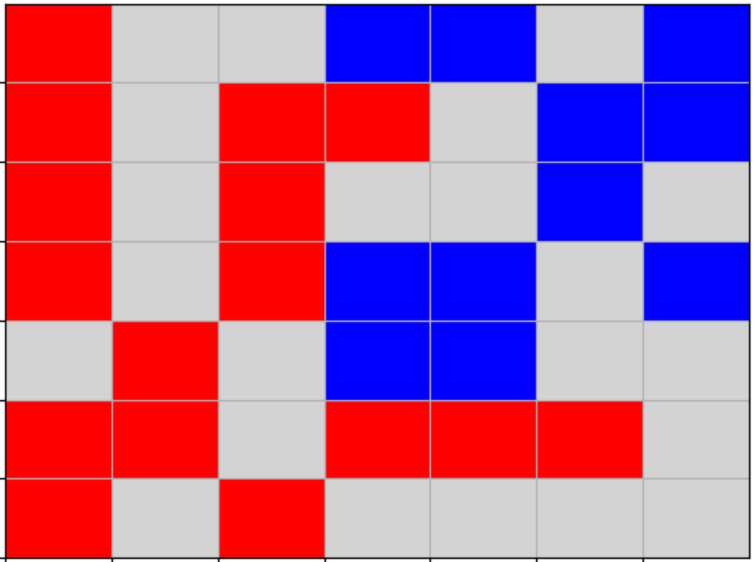
\includegraphics[height=2in]{simple_game.png}
\end{figure}

\begin{figure}[h!]
\centering
  \caption{The duo board}
  \label{fig:duoBoard}
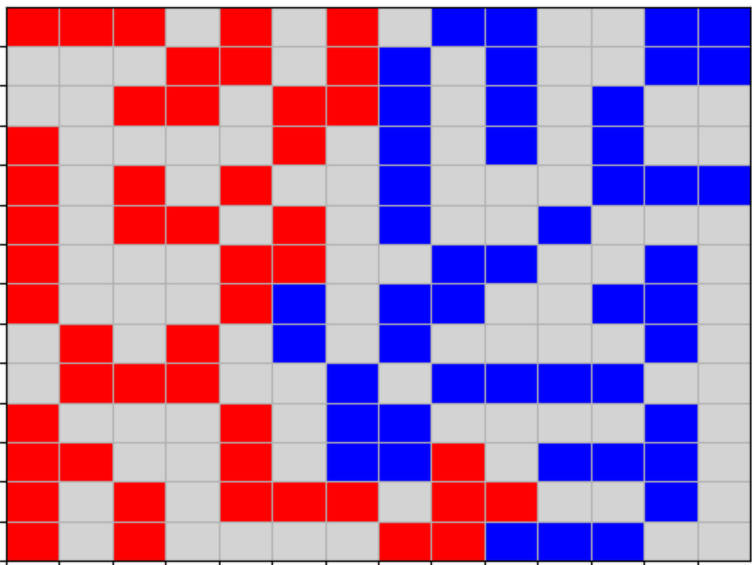
\includegraphics[height=2in]{duo_game.png}
\end{figure}

\begin{figure}[h!]
\centering
  \caption{The hard board}
  \label{fig:hardBoard}
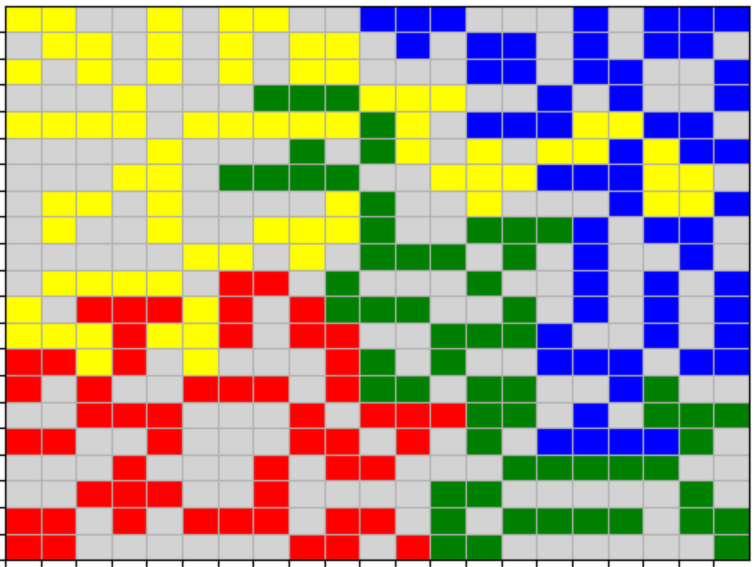
\includegraphics[height=2in]{hard_game.png}
\end{figure}

Every tile can either be the player's id (i.e. 1, 2, 3 or 4) or empty (0). The general formula is then described in \ref{formula:observation}
\begin{align}
\textit{Observations} = \textit{Board Size} \times (\textit{Players} + 1)
\label{formula:observation}
\end{align}

The number of possible actions is a bit more tricky. It is all the possible placements of all the pieces. It can be the 4 rotations (0, 90, 180 and 270 degrees) combined with a flip (either horizontal or vertical) and then placed on all the available translations on the board. Some pieces are harder to calculate than others, but
 it is easier to test all the combinations experimentally and come out with the number as it is shown in \ref{tab:boards} next to the Actions row. The Mean per turn row measures the average number of available moves per turn, the RL agent tries to take the best out of this number per turn. These results come from 100 simulations ran with random agents.
 
\begin{figure}[h!]
\centering
  \caption{The 8 placements for the L4 piece}
  \label{fig:8moves}
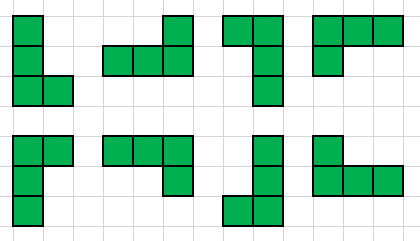
\includegraphics[height=1.5in]{8_moves.png}
\end{figure}

\begin{figure}[h!]
\centering
  \caption{The single placement for the X5 piece}
  \label{fig:singleMove}
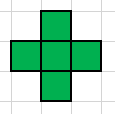
\includegraphics[height=0.75in]{single_move.png}
\end{figure}

Finally, the rewards go as follow:
\begin{itemize}
\item +1 for a win
\item -1 for a lost
\item 0 for a tie
\item 0 for any other move
\end{itemize}
 
\subsection{Model Architecture}

For the production of the electronic manuscript, you must use Adobe's
{\em Portable Document Format} (PDF). A PDF file can be generated, for
instance, on Unix systems using {\tt ps2pdf} or on Windows systems
using Adobe's Distiller. There is also a website with free software
and conversion services: \url{http://www.ps2pdf.com}. For reasons of
uniformity, use of Adobe's {\em Times Roman} font is strongly suggested. In
\LaTeX2e{}, this is accomplished by putting
\begin{quote} 
\mbox{\tt $\backslash$usepackage\{times\}}
\end{quote}
in the preamble.\footnote{You may want also to use the package {\tt
latexsym}, which defines all symbols known from the old \LaTeX{}
version.}
  
Additionally, it is of utmost importance to specify the American {\bf
letter} format (corresponding to 8-1/2$''$ $\times$ 11$''$) when
formatting the paper. When working with {\tt dvips}, for instance, one
should specify {\tt -t letter}.

\subsection{Title and Author Information}

Center the title on the entire width of the page in a 14-point bold
font. The title should be capitalized using Title Case. Below it, center author name(s) in  12-point bold font. On the following line(s) place the affiliations, each affiliation on its own line using 12-point regular font. Matching between authors and affiliations can be done using numeric superindices. Optionally, a comma-separated list of email addresses follows the affiliation(s) line(s), using  12-point regular font.

\subsubsection{Blind Review}

In order to make blind reviewing possible, authors must omit their
names and affiliations when submitting the paper for review. In place
of names and affiliations, provide a list of content areas. When
referring to one's own work, use the third person rather than the
first person. For example, say, ``Previously,
Gottlob~\shortcite{gottlob:nonmon} has shown that\ldots'', rather
than, ``In our previous work~\cite{gottlob:nonmon}, we have shown
that\ldots'' Try to avoid including any information in the body of the
paper or references that would identify the authors or their
institutions. Such information can be added to the final camera-ready
version for publication.

\subsection{Abstract}

Place the abstract at the beginning of the first column 3$''$ from the
top of the page, unless that does not leave enough room for the title
and author information. Use a slightly smaller width than in the body
of the paper. Head the abstract with ``Abstract'' centered above the
body of the abstract in a 12-point bold font. The body of the abstract
should be in the same font as the body of the paper.

The abstract should be a concise, one-paragraph summary describing the
general thesis and conclusion of your paper. A reader should be able
to learn the purpose of the paper and the reason for its importance
from the abstract. The abstract should be no more than 200 words long.

\subsection{Text}

The main body of the text immediately follows the abstract. Use
10-point type in a clear, readable font with 1-point leading (10 on
11).

Indent when starting a new paragraph, except after major headings.

\subsection{Headings and Sections}

When necessary, headings should be used to separate major sections of
your paper. (These instructions use many headings to demonstrate their
appearance; your paper should have fewer headings.). All headings should be capitalized using Title Case.

\subsubsection{Section Headings}

Print section headings in 12-point bold type in the style shown in
these instructions. Leave a blank space of approximately 10 points
above and 4 points below section headings.  Number sections with
arabic numerals.

\subsubsection{Subsection Headings}

Print subsection headings in 11-point bold type. Leave a blank space
of approximately 8 points above and 3 points below subsection
headings. Number subsections with the section number and the
subsection number (in arabic numerals) separated by a
period.

\subsubsection{Subsubsection Headings}

Print subsubsection headings in 10-point bold type. Leave a blank
space of approximately 6 points above subsubsection headings. Do not
number subsubsections.

\paragraph{Titled paragraphs.} You can use titled paragraphs if and 
only if the title covers exactly one paragraph. Such paragraphs must be
separated from the preceding content by at least 3pt, and no more than
6pt. The title must be in 10pt bold font and ended with a period. 
After that, a 1em horizontal space must follow the title before 
the paragraph's text.

In \LaTeX{} titled paragraphs must be typeset using
\begin{quote}
{\tt \textbackslash{}paragraph\{Title.\} text} .
\end{quote}

\subsubsection{Acknowledgements}

You may include an unnumbered acknowledgments section, including
acknowledgments of help from colleagues, financial support, and
permission to publish. If present, acknowledgements must be in a dedicated,
unnumbered section appearing after all regular sections but before any
appendices or references.

Use 
\begin{quote}
    {\tt \textbackslash{}section*\{Acknowledgements\}})
\end{quote}
to typeset the acknowledgements section in \LaTeX{}.

\subsubsection{Appendices}

Any appendices directly follow the text and look like sections, except
that they are numbered with capital letters instead of arabic
numerals. See this document for an example.

\subsubsection{References}

The references section is headed ``References'', printed in the same
style as a section heading but without a number. A sample list of
references is given at the end of these instructions. Use a consistent
format for references. The reference list should not include unpublished
work.

\subsection{Citations}

Citations within the text should include the author's last name and
the year of publication, for example~\cite{gottlob:nonmon}.  Append
lowercase letters to the year in cases of ambiguity.  Treat multiple
authors as in the following examples:~\cite{abelson-et-al:scheme}
or~\cite{bgf:Lixto} (for more than two authors) and
\cite{brachman-schmolze:kl-one} (for two authors).  If the author
portion of a citation is obvious, omit it, e.g.,
Nebel~\shortcite{nebel:jair-2000}.  Collapse multiple citations as
follows:~\cite{gls:hypertrees,levesque:functional-foundations}.
\nocite{abelson-et-al:scheme}
\nocite{bgf:Lixto}
\nocite{brachman-schmolze:kl-one}
\nocite{gottlob:nonmon}
\nocite{gls:hypertrees}
\nocite{levesque:functional-foundations}
\nocite{levesque:belief}
\nocite{nebel:jair-2000}

\subsection{Footnotes}

Place footnotes at the bottom of the page in a 9-point font.  Refer to
them with superscript numbers.\footnote{This is how your footnotes
should appear.} Separate them from the text by a short
line.\footnote{Note the line separating these footnotes from the
text.} Avoid footnotes as much as possible; they interrupt the flow of
the text.

\section{Results}

Place all illustrations (figures, drawings, tables, and photographs)
throughout the paper at the places where they are first discussed,
rather than at the end of the paper.

They should be floated to the top (preferred) or bottom of the page, 
unless they are an integral part 
of your narrative flow. When placed at the bottom or top of
a page, illustrations may run across both columns, but not when they
appear inline.

Illustrations must be rendered electronically or scanned and placed
directly in your document. All illustrations should be understandable when printed in black and
white, albeit you can use colors to enhance them. Line weights should
be 1/2-point or thicker. Avoid screens and superimposing type on
patterns as these effects may not reproduce well.

Number illustrations sequentially. Use references of the following
form: Figure 1, Table 2, etc. Place illustration numbers and captions
under illustrations. Leave a margin of 1/4-inch around the area
covered by the illustration and caption.  Use 9-point type for
captions, labels, and other text in illustrations. Captions should always appear below the illustration.

\section{Analysis}

Tables are considered illustrations containing data. Therefore, they should also appear floated to the top (preferably) or bottom of the page, and with the captions below them.

\begin{table}
\centering
\begin{tabular}{lll}
\hline
Scenario  & $\delta$ & Runtime \\
\hline
Paris       & 0.1s  & 13.65ms     \\
Paris       & 0.2s  & 0.01ms      \\
New York    & 0.1s  & 92.50ms     \\
Singapore   & 0.1s  & 33.33ms     \\
Singapore   & 0.2s  & 23.01ms     \\
\hline
\end{tabular}
\caption{Latex default table}
\label{tab:plain}
\end{table}

\begin{table}
\centering
\begin{tabular}{lrr}  
\toprule
Scenario  & $\delta$ (s) & Runtime (ms) \\
\midrule
Paris       & 0.1  & 13.65      \\
            & 0.2  & 0.01       \\
New York    & 0.1  & 92.50      \\
Singapore   & 0.1  & 33.33      \\
            & 0.2  & 23.01      \\
\bottomrule
\end{tabular}
\caption{Booktabs table}
\label{tab:booktabs}
\end{table}

If you are using \LaTeX, you should use the {\tt booktabs} package, because it produces better tables than the standard ones. Compare Tables \ref{tab:plain} and~\ref{tab:booktabs}. The latter is clearly more readable for three reasons:

\begin{enumerate}
    \item The styling is better thanks to using the {\tt booktabs} rulers instead of the default ones.
    \item Numeric columns are right-aligned, making it easier to compare the numbers. Make sure to also right-align the corresponding headers, and to use the same precision for all numbers.
    \item We avoid unnecessary repetition, both between lines (no need to repeat the scenario name in this case) as well as in the content (units can be shown in the column header).
\end{enumerate}

\section{Conclusion}

IJCAI's two-column format makes it difficult to typeset long formulas. A usual temptation is to reduce the size of the formula by using the {\tt small} or {\tt tiny} sizes. This doesn't work correctly with the current \LaTeX{} versions, breaking the line spacing of the preceding paragraphs and title, as well as the equation number sizes. The following equation demonstrates the effects (notice that this entire paragraph looks badly formatted):
%
\begin{tiny}
\begin{equation}
    x = \prod_{i=1}^n \sum_{j=1}^n j_i + \prod_{i=1}^n \sum_{j=1}^n i_j + \prod_{i=1}^n \sum_{j=1}^n j_i + \prod_{i=1}^n \sum_{j=1}^n i_j + \prod_{i=1}^n \sum_{j=1}^n j_i
\end{equation}
\end{tiny}%

Reducing formula sizes this way is strictly forbidden. We {\bf strongly} recommend authors to split formulas in multiple lines when they don't fit in a single line. This is the easiest approach to typeset those formulas and provides the most readable output%
%
\begin{align}
    x =& \prod_{i=1}^n \sum_{j=1}^n j_i + \prod_{i=1}^n \sum_{j=1}^n i_j + \prod_{i=1}^n \sum_{j=1}^n j_i + \prod_{i=1}^n \sum_{j=1}^n i_j + \nonumber\\
    + & \prod_{i=1}^n \sum_{j=1}^n j_i
\end{align}%

If a line is just slightly longer than the column width, you may use the {\tt resizebox} environment on that equation. The result looks better and doesn't interfere with the paragraph's line spacing: %
\begin{equation}
\resizebox{.91\linewidth}{!}{$
    \displaystyle
    x = \prod_{i=1}^n \sum_{j=1}^n j_i + \prod_{i=1}^n \sum_{j=1}^n i_j + \prod_{i=1}^n \sum_{j=1}^n j_i + \prod_{i=1}^n \sum_{j=1}^n i_j + \prod_{i=1}^n \sum_{j=1}^n j_i
$}
\end{equation}%

This last solution may have to be adapted if you use different equation environments, but it can generally be made to work. Please notice that in any case:

\begin{itemize}
    \item Equation numbers must be in the same font and size than the main text (10pt).
    \item Your formula's main symbols should not be smaller than {\small small} text (9pt).
\end{itemize}

For instance, the formula
%
\begin{equation}
    \resizebox{.91\linewidth}{!}{$
    \displaystyle
    x = \prod_{i=1}^n \sum_{j=1}^n j_i + \prod_{i=1}^n \sum_{j=1}^n i_j + \prod_{i=1}^n \sum_{j=1}^n j_i + \prod_{i=1}^n \sum_{j=1}^n i_j + \prod_{i=1}^n \sum_{j=1}^n j_i + \prod_{i=1}^n \sum_{j=1}^n i_j
$}
\end{equation}
% 
would not be acceptable because the text is too small.

\section{Algorithms and Listings}

Algorithms and listings are a special kind of figures. Like all illustrations, they should appear floated to the top (preferably) or bottom of the page. However, their caption should appear in the header, left-justified and enclosed between horizontal lines, as shown in Algorithm~\ref{alg:algorithm}. The algorithm body should be terminated with another horizontal line. It is up to the authors to decide whether to show line numbers or not, how to format comments, etc.

In \LaTeX{} algorithms may be typeset using the {\tt algorithm} and {\tt algorithmic} packages, but you can also use one of the many other packages for the task.  

\begin{algorithm}[tb]
\caption{Example algorithm}
\label{alg:algorithm}
\textbf{Input}: Your algorithm's input\\
\textbf{Parameter}: Optional list of parameters\\
\textbf{Output}: Your algorithm's output
\begin{algorithmic}[1] %[1] enables line numbers
\STATE Let $t=0$.
\WHILE{condition}
\STATE Do some action.
\IF {conditional}
\STATE Perform task A.
\ELSE
\STATE Perform task B.
\ENDIF
\ENDWHILE
\STATE \textbf{return} solution
\end{algorithmic}
\end{algorithm}

\section*{Acknowledgments}

The preparation of these instructions and the \LaTeX{} and Bib\TeX{}
files that implement them was supported by Schlumberger Palo Alto
Research, AT\&T Bell Laboratories, and Morgan Kaufmann Publishers.
Preparation of the Microsoft Word file was supported by IJCAI.  An
early version of this document was created by Shirley Jowell and Peter
F. Patel-Schneider.  It was subsequently modified by Jennifer
Ballentine and Thomas Dean, Bernhard Nebel, Daniel Pagenstecher,
Kurt Steinkraus, Toby Walsh and Carles Sierra. The current version 
has been prepared by Marc Pujol-Gonzalez and Francisco Cruz-Mencia.

\appendix

\section{\LaTeX{} and Word Style Files}\label{stylefiles}

The \LaTeX{} and Word style files are available on the IJCAI--19
website, \url{http://www.ijcai19.org}.
These style files implement the formatting instructions in this
document.

The \LaTeX{} files are {\tt ijcai19.sty} and {\tt ijcai19.tex}, and
the Bib\TeX{} files are {\tt named.bst} and {\tt ijcai19.bib}. The
\LaTeX{} style file is for version 2e of \LaTeX{}, and the Bib\TeX{}
style file is for version 0.99c of Bib\TeX{} ({\em not} version
0.98i). The {\tt ijcai19.sty} style differs from the {\tt
ijcai18.sty} file used for IJCAI--18.

The Microsoft Word style file consists of a single file, {\tt
ijcai19.doc}. This template differs from the one used for
IJCAI--18.

These Microsoft Word and \LaTeX{} files contain the source of the
present document and may serve as a formatting sample.  

Further information on using these styles for the preparation of
papers for IJCAI--19 can be obtained by contacting {\tt
pcchair@ijcai19.org}.

%% The file named.bst is a bibliography style file for BibTeX 0.99c
\bibliographystyle{named}
\bibliography{ijcai19}

\end{document}



